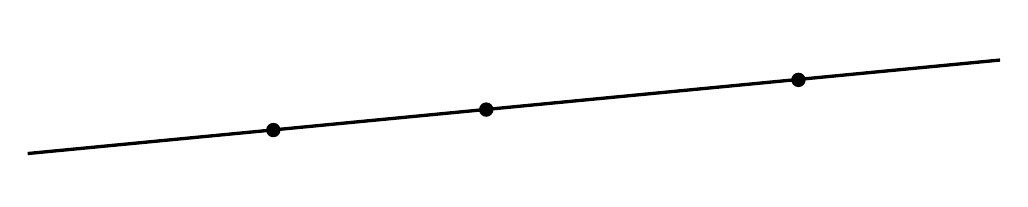
\begin{tikzpicture}[xscale = 1.3, yscale = 1.3]
    \clip(-3.6,1.24) rectangle (5.9,2.72);
    \draw [line width=1.2pt,domain=-3.6:5.9] plot(\x,{(--3.82--0.2*\x)/2.08});
    \begin{scriptsize}
        \fill [color=black] (-1.2,1.72) circle (2.0pt);
        \fill [color=black] (0.88,1.92) circle (2.0pt);
        \fill [color=black] (3.93,2.21) circle (2.0pt);
        \fill [color=black] (9.82,-1.68) circle (2.0pt);
    \end{scriptsize}
\end{tikzpicture}